\documentclass[12pt,leqno,a4paper]{article}


\usepackage{natbib}
\usepackage{epsfig}
\usepackage{booktabs}
\usepackage[paper=a4paper,left=3cm,right=3cm]{geometry}% http://ctan.org/pkg/geometry
\usepackage[utf8]{inputenc} 
\usepackage[english,german]{babel}
\usepackage{dingbat}
\usepackage{amsmath}
\usepackage{amsfonts}
\usepackage{float}
\usepackage[extra]{tipa}
\usepackage{dingbat}
\usepackage{algorithm}
\usepackage{algpseudocode}

% Minimalbeispiel für Diplom- oder Studienarbeit in Latex
% OHNE GEWAEHR
% Antje Schweitzer, Juli 2011 & Juli 2014 
% folgende Dateien gehoeren zu diesem Beispiel:
% - thesis.tex (der eigentliche Text)
% - references.bib (die "Datenbank" mit den Literaturverweisen im Bibtex-Format)
% - example.pdf (eine Beispielgrafik)
% damit kann man dann nach der Anleitung unten folgendes Dokument erzeugen:
% - thesis.pdf 

% Minimal example for student papers in LaTeX, can be used as a template
% without warranty
% (English "translation" by Nils Reiter, July 2014)
% You need multiple files for this example to work:
% - thesis.tex (this file)
% - references.bib (a BibTeX file containing the bibliographic entries)
% - example.pdf (an example figure)

% ANLEITUNG -- INSTRUCTIONS
% To create a PDF, please run the following steps:
% - pdflatex thesis.tex
% - bibtex thesis
% - pdflatex thesis.tex
% - pdflatex thesis.tex
% (yes, some steps need to be run multiple times, for reasons)

% Antje Schweitzer, Oct. 2016 - updated statement of authorship
% 
% Antje Schweitzer, Dec 2020 
% - updated translation of statement of authorship ;)
% - made title fit into the window prescribed for Computer Science theses
% please note that for the Computer Science students, the statements
% have slightly different wordings and need to be on the last page
% please check requirements by C.S. department in that case
% (also no guarantee that the window is correct -
% the version I compiled and printed does fit)
% - changed to UTF-8 encoded .tex file, included inputenc utf8, 
% so Umlauts can be typed as usual

\renewcommand{\baselinestretch}{1.3}
\parskip = \medskipamount
\frenchspacing
\bibpunct[; ]{(}{)}{;}{a}{,}{;}


\newcommand{\Titel}{Phonetic Representations of Speech\\ 
for Human Pronunciation Feedback and Automatic Accent Transfer}

\begin{document}
\begin{titlepage}
    % different margin so titlepage fits into template
    \newgeometry{left=3.5cm,right=2cm}
    \large
     \begin{center}
      Institut für Maschinelle Sprachverarbeitung\\
      Universität Stuttgart\\
      Pfaffenwaldring 5B\\
      D-70569 Stuttgart\\    
      
      \vspace{2.5cm}
      Master thesis\\
     % \vfill
      {\LARGE \bf \Titel} \\
      \vspace{2cm}
      Isaac Riley\\
         \vfill
      \begin{tabular}[t]{lr}
      Studiengang: & M.Sc. Computational Linguistics \\ % oder: B.Sc. Maschinelle Sprachverarbeitung, M.Sc. Informatik, ...\\
      \\
      \\
      {Prüfer*innen:} & Prof. Dr. Wolfgang Wokurek\\
       & Prof. Dr. Antje Schweitzer\\
      {Betreuer:} & Prof. Dr. Wolfgang Wokurek\\ 
      \\
      \\
      {Beginn der Arbeit:} & 06.04.2021\\
      {Ende der Arbeit:} & 06.10.2021\\
      \end{tabular}
    \end{center}
  \setlength{\hoffset}{0cm}
    \normalsize
  \end{titlepage}
  \newgeometry{left=3cm,right=3cm}
  
  \newpage
  \thispagestyle{empty}
  \begin{otherlanguage}
  {german}
  \noindent\textbf{Erklärung (Statement of Authorship)}\\
  
  
  \noindent Hiermit erkläre ich, dass ich die vorliegende Arbeit selbstständig verfasst habe und dabei keine andere als die angegebene Literatur verwendet habe. Alle Zitate und sinngemäßen Entlehnungen sind als solche unter genauer Angabe der Quelle gekennzeichnet. Die eingereichte Arbeit ist weder vollständig noch in wesentlichen Teilen Gegenstand eines anderen Prüfungsverfahrens gewesen. Sie ist weder vollständig noch in Teilen bereits veröffentlicht. Die beigefügte elektronische Version stimmt mit dem Druckexemplar überein.%% delete the following for theses in German; 
  %% delete or keep for English theses. 
  %% The German version above must be retained 
  %% and signed even if the thesis is written
  %% in another language than German.
  \end{otherlanguage}
  \footnote{Non-binding translation for convenience: This thesis is the result of my own independent work, and any material from work of others which is used either verbatim or indirectly in the text is credited to the author including details about the exact source in the text. This work has not been part of any other previous examination, neither completely nor in parts. It has neither completely nor partially been published before. The submitted electronic version is identical to this print version.}\\[2cm]
  \vspace{2cm}
  (Isaac Riley)
  
  \newpage
  \thispagestyle{empty}
  \noindent \textbf{Acknowledgments}\\
  \noindent I wish to express my thanks to Dr. Wokurek for his mentoring and encouragement. 
  He was incredibly generous with his time, and his advice and willingness to listen 
  to my ideas helped me to keep a level head throughout what was at times a difficult 
  research process. I learned from him more than he may suspect, and I will carry his 
  insights and advice with me long after I have submitted my thesis.
\\~\\
  I am eternally indebted to my wife, Sandra, for her assistance and 
  encouragement. 
  In so many ways, she made this possible.
  To her I owe not only my thesis, but also my sanity.
  %I would like to thank my friends for their feedback and encouragement 
  %throughout the entire process. 
  
  
  \newpage
  {\selectlanguage{english}\tableofcontents}
  \newpage
\section{Introduction [4]}
  In linguistics, the notion of accent refers to a pattern of pronunciation that does not change 
the semantic content of what is uttered, but which may carry pragmatic meaning and 
convey demographic information about the speaker. While some phonetic variation may be random 
or occur at the individual level (idiolect), accent typically varies systematically according 
to native language and dialect, which in turn vary geographically and demographically.

Accent is occasionally an impediment to human understanding of speech; however, among native 
and advanced speakers, accent is often no impediment to communication.
In automatic speech recognition, accent accents underrepresented in training datasets 
typically have a much stronger negative effect on recognition accuracy. For this reason, 
accent is an active subject of research in automatic speech processing.
%accent transfer and reduction
%accent recognition
%voice conversion and voice cloning

Related to accent transfer is the task of voice conversion. The goal of voice conversion is to 
generate speech containing identical linguistic information as an input sample, modifying only the 
timbre to match a target speaker. In some respects, voice conversion is a simpler task; namely, 
there is no temporal realignment and phonetic information remains the same. 
The absence of temporal realignment means that voice conversion models have an equal number of frames 
in input and output. This makes possible frame-to-frame mappings, also surrounding context must still 
be taken into account in order to achieve good results.

This works explores approaches to accent conversion with and without voice conversion. 
These approaches may be referred respectively as intra-speaker accent conversion and cross-speaker 
accent conversion.
In intra-speaker accent conversion (henceforth simply \textit{accent conversion}), an utterance from the source speaker is modified to match the accent 
of the target speaker, without changing voice quality or non-accent-carrying linguistic content. 
By contrast, in cross-speaker accent conversion, accent conversion is combined with voice conversion. Henceforth, this will 
simply be referred to as speaker conversion.

This work investigates two distinct but related approaches to speech conversion, both accent conversion and 
speaker conversion. The first is a continuous approach in which speech is mapped to and synthesized from a
continuous phonetic representation. The second is a discrete approach, in which speech is transcribed to and 
synthesized from the International Phonetic Alphabet (IPA).

Clearly, in the simplest case, speaker conversion may involve the combination of ASR and TTS, where the ASR model 
recognizes the speech of the source speaker and the TTS model synthesizes the speech of the target speaker from that same text.
This work takes an alternative approach, in which speech is transcribed in the IPA, 
modified by an intermediate model to match the phonetic patterns of the target speaker, and a TTS model trained 
to synthesize speech from IPA is used to synthesize the desired speech.

\begin{center}
  \textbf{Summary and Comparison of Speech Conversion Tasks}\\~\\
  \begin{tabular}{l|c|c|c}
    %\caption{Intra-Speaker Accent Conversion}
      Speech Aspect   & Accent Conversion & Voice Conversion & Speaker Conversion \\\hline
      content         & source & source & source \\
      accent          & \textbf{target} & source & \textbf{target} \\
      vocal quality   & source & \textbf{target} & \textbf{target} \\
    \end{tabular}
  \end{center}

\section{Background [9]}
    \subsection{Automatic Speech Recognition [2]}
        

    \subsection{Text-to-Speech Synthesis [1.5]}
        As its name suggests, test-to-speech synthesis involves generating waveform speech from text input. 
State-of-the art approaches are typically neural and involve a feature prediction network (FPN) and 
and audio generating network (AGN).

*** STILL NEED TO TYPESET REST OF NOTES ***

    \subsection{Speech Signal Processing [1.5]}
        Time-domain representations of signals are not ideal for most speech processing 
algorithms. To render speech more tractable, it is converted to the frequency domain, 
which allows a more compact representation, and one containing more information that 
is directly pertinent to the task of speech recognition.

\subsubsection{Short-Time Fourier Transform}

The favored approach to conversion from the tme domain to the frequency domain is the 
discrete-time short-time Fourier transform (STFT), which is given by 
$$\textbf{STFT}\{ x[n] \}( m, \omega ) := %X(m, \omega) = 
\sum\limits_{n=-\infty}^{\infty} x[n] w[n-m] e^{-j \omega m}$$
for some signal $x[n]$, windowing function $w[n-m]$, and frequency $\omega$.

To avoid discontinuities between frames, i.e. between adjacent spectra, the window 
function advances across the signal at some fixed shift, which is less than the 
width of the window; in other words, the windows overlap. 

To obtain the (power) spectrogram, the squared magnitude of each element is taken 
and the resulting discretized spectra are concatenated to form a matrix. 
Because this operation discards phase information, it is not lossless. As a result, 
a major task of speech synthesis from spectrograms is to reconstruct the phase.
A sample spectrogram is shown below:

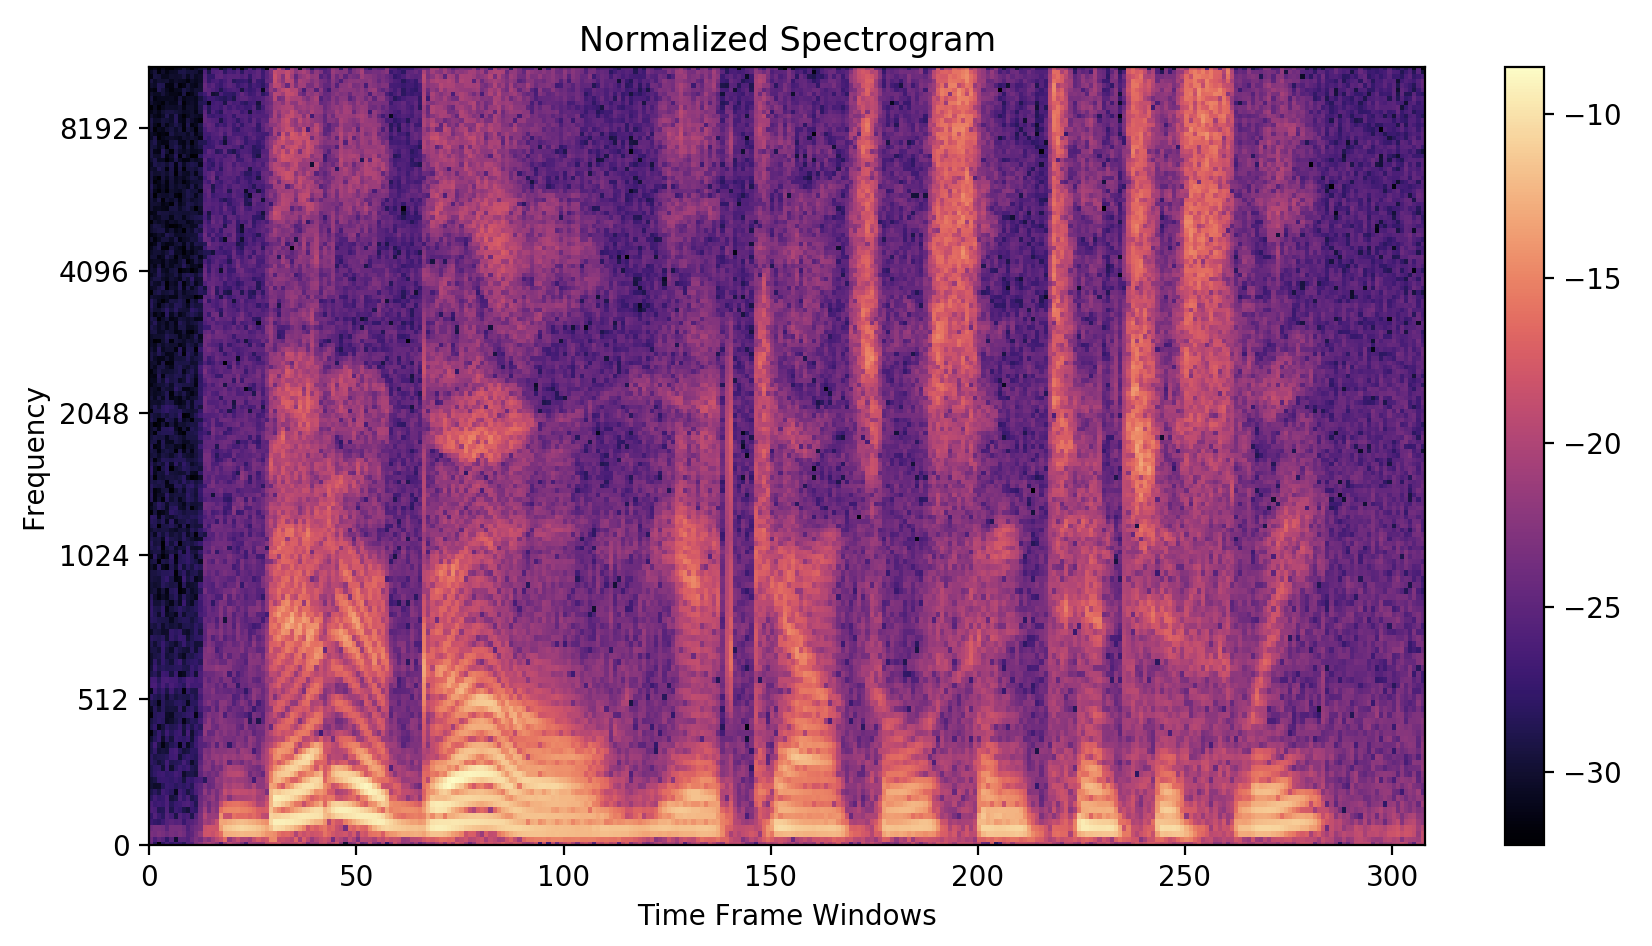
\includegraphics[width=\textwidth]{img/img_spectrogram.png}


%https://www.youtube.com/watch?v=UKHBWzoOKsY

\subsubsection{Mel Spectrum and Coefficients}
%https://en.wikipedia.org/wiki/Mel-frequency_cepstrum
%https://en.wikipedia.org/wiki/Mel_scale
%http://practicalcryptography.com/miscellaneous/machine-learning/guide-mel-frequency-cepstral-coefficients-mfccs/
%https://medium.com/analytics-vidhya/understanding-the-mel-spectrogram-fca2afa2ce53
%https://towardsdatascience.com/getting-to-know-the-mel-spectrogram-31bca3e2d9d0
%https://de.wikipedia.org/wiki/Mel_Frequency_Cepstral_Coefficients
%https://towardsdatascience.com/extract-features-of-music-75a3f9bc265d
%https://medium.com/analytics-vidhya/understanding-the-mel-spectrogram-fca2afa2ce53

A well-established finding from psychoacoustics is that human perception of sounds is not linear 
in frequency. Differences at lower frequencies are perceived as sounding `further apart' 
than the same absolute difference at higher frequencies. To reflect this, speech is mapped nonlinearly 
onto the mel scale
$$M(f) = 1125 \ln (1 + f/700)$$ 
typically using overlapping triangular windows whose spacing reflects human perception. 

To obtain the mel-frequency cepstrum, a number of additional operations are performed \citep{mel2012}.
At each of the mel frequencies, the log is taken of the power, which reflects the non-linear 
human perception of loudness.
Finally, the Discrete Cosine Transform of these values gives the mel-frequency cepstral coefficients, 
which together make up the mel frequency cepstrum.

%\subsubsection{}
%\subsubsection{}
    \subsection{Neural Networks [3]}
        %According to a popular aphorism, ``two heads are better than one.'' 
%One may suppose, inductively reasoning, that three heads are likewise better than two, 
%and so on. It seems reasonable to suppose that, due to the principle of diminishing returns
Neural networks are, most generally, a powerful application of the ensemble 
approach to machine learning in which simple units (``nodes'') are joined together to learn 
complex functions \citep{aggarwal}. Originally inspired by the structure of the human brain, 
the degree to which this comparison is warranted remains controversial; nevertheless, 
the terminology is still used today.

At its core, a neural network consists of a series of linear and nonlinear operations 
that may be combined in various ways. Like other machine learning algorithms, 
an input is mapped to an output. However, a key advantage of neural networks is their ability 
to learn features internally. 

Training is performed by means of the backpropagation algorithm, which makes possible 
the correct attribution of error to each parameter. The parameters are updated proportionally 
to their contribution to the error.

%\subsubsection{Feedforward Neural Networks}
The simplest kind of neural network, the feedforward neural network (FFNN), consists of an 
\textit{input layer}, zero or more \textit{hidden layers}, and an \textit{output layer}, 
where each hidden layer and optionally the output layer is passed to a nonlinear activation 
function such as $\sigma(x) = \dfrac{e^x}{1+e^x}$ or $\tanh(x) = \dfrac{e^x - e^{-x}}{e^x+e^{-x}}$. 
The activation function makes it possible to learn complex functions, since without it 
a feedforward neural network would always be equivalent to multiplication by a matrix.

\subsubsection{Recurrent Neural Networks}
Feedforward neural networks are effective in processing vector inputs. If the  
data possess a sequential nature, a FFNN may struggle to learn the intertemporal 
relationships. To solve this problem, the recurrent neural network was proposed, in which 
at each time step, the network's output from that time step is passed as input to the network at 
the current time step. Notationally, given an input vector $x$ at time $t$,
$$h(x_t) = f(h_{t-1}, x_t; \theta)$$
$$a_t = W^{(h \rightarrow h)} t_{t-1}+W^{(x \rightarrow h)} x_t + b$$
$$h_t = \tanh(a_t)$$
$$o_t = W^{(h \rightarrow o)}h_t + c$$
%$$\hat{y}_t = \textrm{softmax}(o_t)$$
%pg 385 of https://www.deeplearningbook.org/contents/rnn.html
where $f$ is the function computed by the RNN \citep{dlbible}. It is important that the loop inherent 
in the architecture of an RNN enables it to handle variable-length input well, which 
is an invaluable property in language- and speech-based settings where input and 
output length tend to vary.

One powerful and popular architecture for recurrent neural networks is the long
short-term memory (LSTM) network \Citep{lstm1997}. One of the problems with simple RNNs is the difficulty 
of modeling long-term dependencies, and more generally with learning which information 
should be passed on (`remembered') and which information should be `forgotten'. To remedy 
this, the LSTM adds a forget gate to regulate which information is passed on in the hidden 
state. 
$$f_t = \sigma(W_f \cdot [h_{t-1}, x_t] + b_f)$$
$$i_t = \sigma(W_i \cdot [h_{t-1}, x_t]+b_t)$$
$$\tilde{C}_t = \tanh (W_C \cdot [h_{t-1}, x_t]+b_C)$$
$$C_t = f_t * C_{t-1} + i_t * \tilde{C}_t$$
$$o_t = \sigma (W_o [h_{t-1}, x_t]+b_o)$$
$$h_t = o_t * \tanh (C_t)$$
%https://colah.github.io/posts/2015-08-Understanding-LSTMs/
The notation followed here is based on that of \cite{olah2015} and \cite{lstmtutorial}

%https://medium.com/@jianqiangma/all-about-recurrent-neural-networks-9e5ae2936f6e

\subsubsection{Sequence-to Sequence Architectures}
A single RNN is well-suited to learning to classify an entire sequence or each 
time step of a sequence; in these respective settings, output size is fixed or 
equal to the input size. However, there are often settings in which input size and 
output size may differ and each varies. In such cases, a sequence-to-sequence model 
is used, in which two RNNs, often two LSTMs, are used.
\citep{dlbible}

\subsubsection{Attention Mechanism}
While LSTMs represent a considerable improvement over vanilla RNNs for a variety of tasks, 
they are far from perfect. 
One difficulty is the inherent difficulty of learning what to remember and what to forget.
State information must be contained in a fixed-length vector. 
The attention mechanism circumvents this bottleneck by adding a sort of query mechanism 
by which the decoder has access to all hidden states of the encoder and learns weights to 
create a weighted sum, which is then used by the decoder to generate the output.
This access to the entire input sequence allows the decoder to focus its `attention', 
as it were, on the most relevant portions of the input, hence the name.
This also brings the added benefit that the alignment between input and output 
can be examined and visualized.

\subsubsection{Convolutional Neural Networks}
When input data have a spatial component, it is beneficial to use a network architecture 
that can take advantage of spatial relationships in the data. A convolutional neural network 
does this by passing a $k \times l$-dimensional filter over the input. 
This is equivalent to a fully-connected network in which a majority of weights are zero.
The relative sparsity of convolutional network networks (CNNs) is one advantage; the primary 
benefit is the ability, given multiple layers, to learn features that correspond to image 
features at various levels of resolution.

\subsubsection{Generative Adversarial Networks}
Operating within the parradigm of supervised learning, neural networks
can be used for classification by learning a posterior distribution over 
labels, given numerical features representing features of an input sample.
%The model is trained by backpropagation, in which errors in classification 
%are appropriately attributed to each of its parameters.
Given sufficient exposure to labeled training data, an appropriately designed 
model can update its parameters so as to assign an increasingly larger probability
to the correct label.

Another branch of machine learning involves generative learning. Given a training dataset,
a generative model learns to output samples resembling those from the training dataset. 

In ``vanilla'' generative adversarial networks (GANs), the are two networks whose training 
takes the form of a minimax game, in which each model seeks to maximize the loss of the other.
The first network is the generator, which is given random noise as input and tasked with 
outputting samples of the same type as the target data. The second model is the discriminator,
a classification network tasked with classifying generated samples as real or generated. 
Throughout the (ideal) adversarial training process, the generator continually improves to 
generate increasingly realistic outputs, and the discriminator becomes increasingly adept at 
distinguishing real samples from generated samples.
    \subsection{International Phonetic Alphabet [1]}
        In natural human language, the correspondence between orthography and pronunciation 
is not entirely one-to-one; in some languages, such as English or Tibetan, it is 
difficult to predict pronunciation from spelling and vice versa. In some languages, 
such as Spanish or Swahili, there is a significantly higher degree of predictability, 
but the dialectical variation means that this tight correspondence does not hold for 
all groups of speakers. Additionally, even among languages using the same scripts, 
the same character often represents differents sounds in different languages. However, 
even within a language, characters can represent different speech sounds depending on 
surrounding letters or position within a word.

For all of these reasons, it is important to have an agreed-upon convention for 
representing speech sounds. The de facto standard is the International Phonetic Alphabet 
\citep{ipa,handbookofphonetics}, 
which was developed to provide a language-agnostic (as well as dialect-agnostic) means 
for phonetic transcription.
This makes it an excellent tool for transcribing accents in which differences in pronunciation 
are of interest.

The IPA is conceived to be able to represent, in theory, all phones appearing in any 
known language, or indeed, any phone realizable by humans. In the present work, because 
the language under consideration is English (albeit with two starkly differing accents), 
the full power of the IPA is not required. All segments considered are either vowels 
or consonants, and all consonants are pulmonic, i.e. produced by exhaling air from the lungs.

Vowels are classified along three key dimensions: openness/closeness, backness/frontness,
and roundedness. The latter is binary, while the other two are continuous.
Consonants are classified by place of articulation, manner of articulation, and voicedness. 
For example, \textipa{b} is the voiced bilabial plosive, while \textipa{p} is its unvoiced 
counterpart. Realized at a different place of articulation, \textipa{g} and \textipa{k} 
are the velar plosives (also respectively voiced and unvoiced). 
Alternatively, holding the place of articulation constant and changing the manner of 
articulation to fricative yields the pair \textipa{B, F}. All phonetic segments used in this work fit this schema.
\section{Related Work [8]}
    \subsection{Prior Work on Accent Transfer [2]}
        Much of the work in accent conversion has been focused on foreign accent conversion,
in which a non-native accent is modified to more closely resemble a native accent.
This has obvious practical applications, but is also important in automatic speech recognition,
since the best-performing models are typically trained on high-resource accents.

All approaches can be divided into parallel and non-parallel approaches, 
as in the related setting of voice conversion.
In parallel accent conversion, data is available which contain identical utterances from
source and target speakers, which in non-parallel accent, the content of the utterance 
need not coincide. There are many advantages inherent in parallel approaches, but 
as parallel data is difficult to collect, it is often less practical. Non-parallel 
data is abundant, but presents another set of challenges, namely the inability to 
use supervised learning approaches. In other words, for a given source utterance, 
there is no correspondending `label' indicating how that same utterance should sound
following conversion. Thus, non-parallel approaches are forced to rely on 
distribution-matching techniques.

%voice morphing
One simple approach is to combine the source and target utterance in some way. 
While somewhat crude in some ways, and arguably not `pure' accent conversion as 
defined above, it nevertheless succeeds in reducing perceived foreign accent. 
However, the output contains characteristics of both the source and target utterance
\citep{voicemorph}.


%frame-pairing
A non-parallel approach is to map frames in the respective utterances into a common phonetic 
space using an aoustic model and then identify the frames of the target speaker that 
are phonetically the most similar to the reference source frame, 
using some similarity metric such as Kullback-Leibler divergence. 
This is an elegant and efficient approach; however, it suffers from a number of drawbacks.
It is unable to handle differences in length between source and desired target, e.g. when 
a segment or sequence of segments typically occupies more frames in one speaker than another.
It also constrains the target space to phones that are in fact realized by the target speaker, 
which may result in partial accent conversion.
Despite these limitations, frame pairing has achieved some success and is a good baseline 
approach
%Using phonetic posteriorgram based frame pairing for segmental accent conversion
%Accent conversion using phonetic posteriorgrams
\citep{framepairing,acppgzhao}.

%articulatory synthesis
The third of the popular parallel approaches involves measurements from an electromagnetic 
articulograph. These are mapped to articulatory features, typically including MFCCs, using a GMM.
The acoustic features are then normalized and provided as input to a appropriate vocoder such as STRAIGHT.
%Accent conversion through cross-speaker articulatory synthesis
\citep{artsynth1}.
However, articulatory approaches are generally found to be inferior to acoustic-based approaches,
which is due in part to the fact that acoustic methods provide a more fine-grained 
representation with which to work.
\citep{artsynth2}.
%


%synthesis-based methods
Another class of accent conversion methods involves those in which speech synthesis 
plays the primary role, typically by representing speech in a shared intermediate 
representation and using a synthesizer trained on speech data of the target speaker 
or accent. One of these, \cite{facviappg}, will be discussed below in greater detail.



%Parrotron: An end-to-end speech-to-speech conversion model and its applications to hearing-impaired speech and speech separation
Another synthesis-based accent conversion model is Parrotron, which makes heavy use 
of both ASR and TTS models. 
Designed to make human communication as well as the use of ASR systems easier for individuals with speech impairments
or strong accents, Parrotron uses transfer learning to adapt a pretrained , already 
robust ASR model to a particular speaker, learning the patterns of errors occurring in 
the individual's speech. This model is then able to transcribe the speech with reasonable accuracy,
which is then synthesized using a pretrained speech synthesis model. While this does 
not preserve voice quality, it does solve the problem of low intelligibility
\cite{parrotron}.



%voice conversion
Voice conversion is task that is in some ways closely related to accent conversion.
In a sense, it may be thought of as a reverse, in that accent conversion generates 
an utterance with the same voice as and a different accent than the source utterance.
In contrast to this, voice conversion generates an utterance with the same accent 
and different voice. Voice conversion is traditionally nearly always performed on 
mel spectrograms, although some progress has been made on waveform-to-waveform 
conversion.









%English Language Accent Classification and Conversion using Machine Learning
%\cite{parikh2020english}

%A new approach to accent recognition and conversion for mandarin chinese
%\cite{ai2020new}

%Accent neutralization for speech recognition of non-native speakers
%\cite{radzikowski2019accent}

%Accent modification for speech recognition of non-native speakers using neural style transfer
%\cite{radzikowski2021accent}

%Hidden Markov Models for Artificial Voice Production and Accent Modification
%\cite{coto2016hidden}

%Foreign Accent Conversion by Synthesizing Speech from Phonetic Posteriorgrams
%\cite{facviappg}


%Improving accent conversion with reference encoder and end-to-end text-to-speech
%\cite{acreference}

%SautiLearn: improving online learning experience with accent translation
%\cite{sautilearn}

%TTS skins: Speaker conversion via ASR
%\cite{ttsskins}


    \subsection{Models Used [6]}
        \subsubsection{Tacotron 2}
Tacotron 2 is a deep neural sequence-to-sequence model that generates mel spectrograms from text. 
I can be combined with a deep neural vocoder, it forms an end-to-end text-to-speech system.
\subsubsection{WaveGlow}
%https://medium.com/subex-ai-labs/understanding-normalizing-flows-and-its-use-case-in-speech-synthesis-part-1-5f805c2d43ce
%https://medium.com/subex-ai-labs/understanding-normalizing-flows-and-its-use-case-in-speech-synthesis-part-2-3e19840e80b5
%https://www.youtube.com/watch?v=B3WlTVvdI5M
%
WaveGlow is a deep neural vocoder that generates waveform audio from mel spectrograms \citep{waveglow}. It has a 
flow-based architecture that learns an invertible mapping, converting a noise vector and 
additional conditioning input into nearly human-sounding waveform audio. Its audio generation 
is accomplished by sampling from a distribution, which is transformed as it passes through the model 
and is conditioned on mel-spectrograms representing the audio that is to be output in waveform.

It is based on the Glow architecture for image generation \citep{glow} and on WaveNet, the groundbreaking 
autoregressive waveform generation model \citep{wavenet}. Its primary advantage over WaveNet is faster inference speed;
because it is non-autoregressive, it can generate audio much faster than WaveNet, and 25 times faster 
than real time on a V100 GPU [XX].

%Its basic architecture is illustrated below:\\
%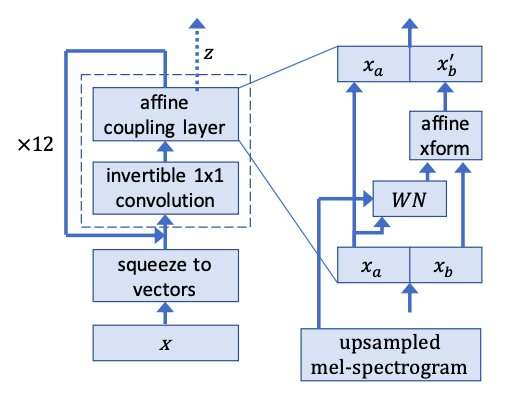
\includegraphics[width=15cm]{img/img_waveglow.jpg}

%Note that much of the computational work is done repetitively, the convolutional and subsequent 
%affine coupling layer are repeated 12 times to generate the level of fine-grained detail 
%required in high-quality waveform.


\subsubsection{CycleGAN}
As described above, in `vanilla' Generative Adversarial Networks, the input is typically random noise, which is mapped to some point in the 
target distribution. Moreover, because the generator is rewarded simply for generating some output 
appearing to have been drawn from the target distribution, there is no direct control over which 
point from the target distribution is generated.
However, there are many applications in which one might wish to exert more control over the output 
by conditioning on some desired criteria. One common case involves the task of image translation,
in which certain aspects of an image are altered while others remain intact. A simple example of 
image translation is a model that transforms horses into zebras. In this case, a simple GAN may take 
a horse image as input and output a very dissimilar zebra image as output; this is because there 
is no constraint to enforce content preservation.
CycleGAN \citep{cycleganvc} achieves this by training an inverse generator to map the transformed image back to the 
original. This cyclical consistency constraint requires the forward generator to preserve semantic 
content from the original image so that it the original can be reconstructed from the transformed image.

\subsubsection{MelGAN-VC}
Most work on GANs focuses on data with a fixed output shape, where 
input size and output shape are typically equal, such as in the case of image generation. 
When an input is supplied, it is for the purpose of conditioning the output and the input 
typically has the same shape as the output.

In settings where the data has an intrinsically sequential nature and the input size varies, 
it is not possible to require a fixed and shape. One such setting is voice conversion, and one 
simple and effective solution has been proposed by Marco Pasini in [XX], illustrated below:\\
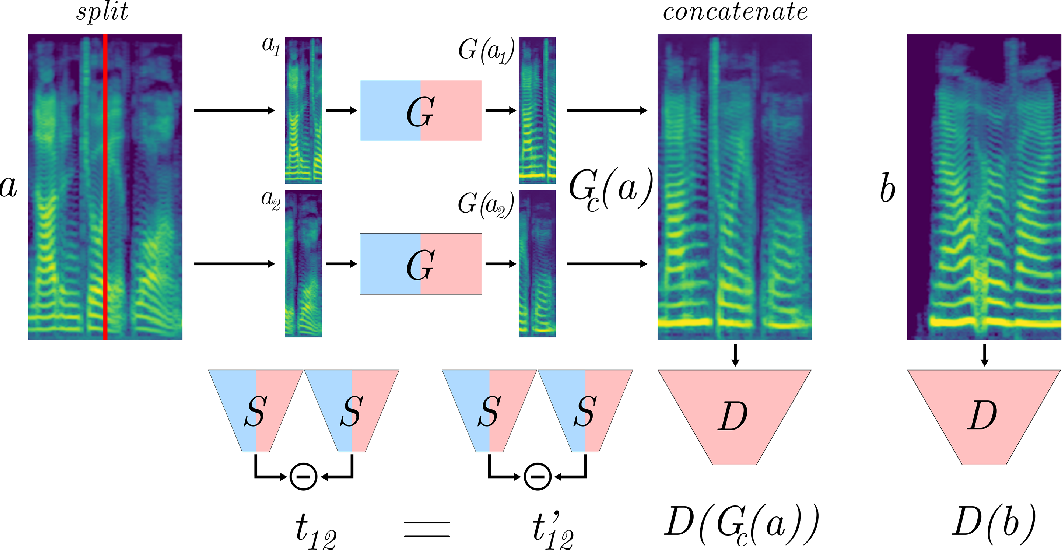
\includegraphics[width=\textwidth]{img/img_melganvc.png}

The key insight is that by taking a fixed length ($T$ frames) of the input spectrogram, 
then splitting the input into two equal-sized blocks and passing each to the generator network. 
The converted spectrograms, i.e. the two generator outputs are then recombined and passed 
to the discriminator. Due to the adversarial loss training objective, the generator must learn 
to convert each block in such a way that, when reassembled, it will be indistinguishable from 
a real sample from the target set. Because the target set does not contain spectrograms with 
discontinuities, such a discontinuity at the splitting point would clearly identify a fake sample. 
Thus, the generator is incentivized to produce outputs which, when re-joined, do not contain 
such telltale discontinuities at the splitting points. Because this applies to any  split point, 
it is possible to train a relatively small generator that can receive inputs of arbitrarily length 
one block at a time and generate the desired output.

\iffalse
\subsubsection{Reinforcement learning and the REINFORCE Algorithm}
Reinforcement learning is a paradigm of machine learning that is well-suited to settings in which an agent 
interacts with an environment and receives rewards as a function of its actions. The objective is to 
choose actions so as to maximize long-term reward. Thus, reinforcement learns a policy, a mapping from 
state to action. The optimal policy yields the maximum expected long-term reward.

There are several different families of approaches in reinforcement learning. 

The REINFORCE algorithm  

\subsubsection{SeqGAN and StepGAN [2]}
Soon after their initial introduction in 2014, GANs achieved remarkable successes in image generation. 
Unfortunately, the GAN framework proved somewhat more difficult to apply to natural language, primarily 
because its gradient-based methods do not work for discrete-valued sequences. To remedy this, 
XXX introduced SeqGAN, an adaptation of GANs to the setting of discrete-valued sequences.

SeqGAN uses the REINFORCE algorithm for training. 
\fi

\subsubsection{Allosaurus}
Allosaurus is a Python library containing tools for automatic neural phonetic transcriptions 
using IPA \Citep{allosaurus}.
Released by a team of researchers at Carnegie Mellon University, it performs phone recognition, 
rather than the more typical task of phoneme recognition, and its main innovation is its so-called 
``allophone layer''. This is a phone-to-phoneme mapping that restricts the phonetic invntory to 
that of a single language. This enable Allosaurus to capture the benefits both of shared phoneme 
models and private phoneme models. While all three architectures use an encoder, shared phoneme models 
use a common phone layer across languages, while in the private phoneme model, each language 
has a separate model following the shared encoder. Allosaurus strikes a balance by using a shared 
decoder or ``universal phone layer'' and leaving the per-language customization to the allophone layer. 
This allows the decoder to benefit from larger amounts of training data and greater generality.
These differences in architecture are shown below:
\begin{center}
  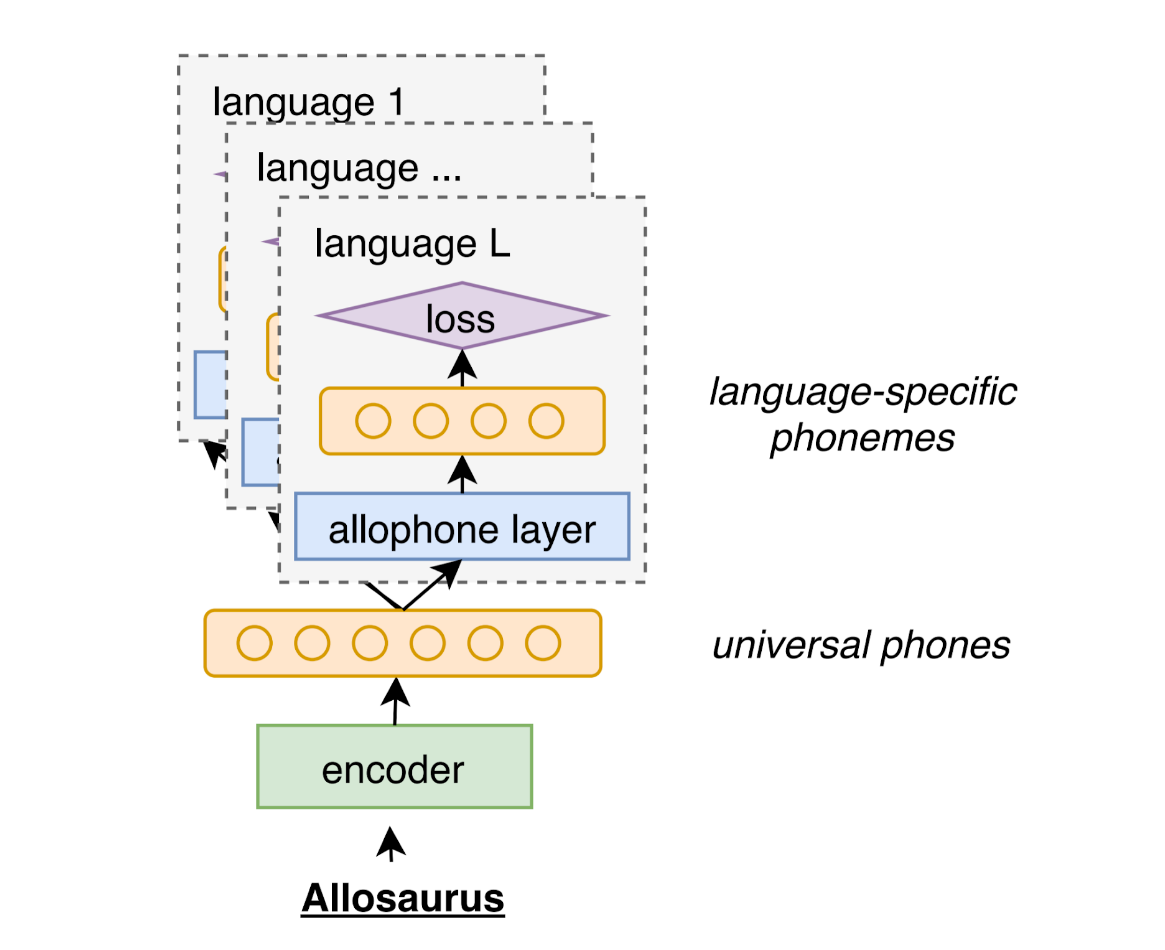
\includegraphics[width=7cm]{img/img_alloraurus.png}
\end{center}

\cite{ctc}

%http://www.scholarpedia.org/article/Policy_gradient_methods#Likelihood_Ratio_Methods_and_REINFORCE
%http://www.scholarpedia.org/article/Policy_gradient_methods#Likelihood_Ratio_Methods_and_REINFORCE
%https://lilianweng.github.io/lil-log/2018/02/19/a-long-peek-into-reinforcement-learning.html
%https://lilianweng.github.io/lil-log/2018/04/08/policy-gradient-algorithms.html
%https://www.quora.com/What-is-the-REINFORCE-algorithm
%
%
%
%
        \newpage
\section{Methods} % [8]
    \subsection{Phonetic Continuous Representation-Based Speech Synthesis and Accent Transfer [3]}
        \subsubsection{Phonetic Posteriorgrams}
A phonetic posteriorgram represents predicted framewise phoneme probabilities from a speech sample.
In this work, a pretrained acoustic model from [XX] was used, due to the high quality of the model, which had 
been trained on the extremely large and varied LibriSpeech corpus.

The acoustic model predicts 5816 senones; the dimensionality is greatly reduced by a linear discriminant 
analysis matrix, yielding the posterior probability for the 40 phonemes in the TIMIT reduced phoneme set, 
which include a silence phoneme (not a true phoneme, but essentially treated as one). Refer to the Data section for samples.


\subsubsection{Speech Synthesis from PPGs [1]}
%Text here.
To generate a mel spectrogram representation from a PPG, a modified version of Tacotron2 
was used. This worked followed NVIDIA's open-source implementation with a few modifications.
As in [XX], and as shown below, the key differences were the addition of a localized attention constraint,
which decreases the computational complexity. This is especially attractive in this case because 
the expected alignment between PPG and mel spectogram is tighter than the alignment between 
text and mel spectrogram (e.g. in the standard Tacotron2 model). Because of this, it is 
superfluous to query all encoder states.

The other important difference is that instead of an embedding layer for the input, a 
linear projection is used, since the input is not sparse, i.e. not one-hot encoded. Thus, 
each input dimension must be taken into account by the model.
The following image summarizes the architecture [XX]:

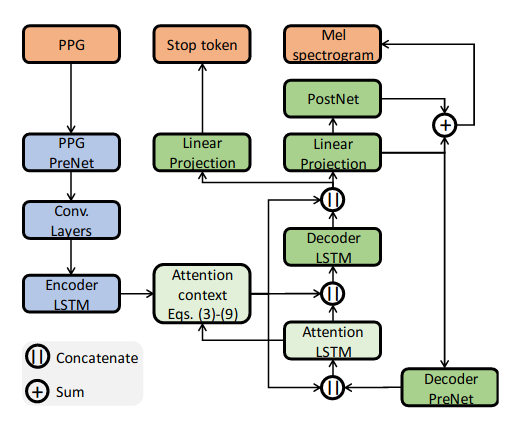
\includegraphics[width=15cm]{img/img_ppg2mel.png}


\subsubsection{Accent Transfer in PPG Space [2]}
%Text here.
Inspired by the basic architecture of MelGAN-VC, the PPG accent transfer model uses a 
generative adversarial network with a cyclical consistency constraint. 
There are two different variants.

The first architecture is convolutional, using one-dimensional convolutions across time. 
Two-dimensional convolutions were not used because there are no local spatial relationships 
across phonemes in a PPG; phoneme oder is not meaningful. The spatial relationships of interest are 
exclusively temporal. 

The second architecture is sequential, a bidirectional LSTM. Each of these 
architectures, when used, is used in both the discriminator and the generator.

*** ILLUSTRATION TO COME ***
    \subsection{Phonetic Transcription-Based Speech Synthesis and Accent Transfer}
        \subsubsection{Relational Mappings for Segmental Accent Transfer [1]}
Because accents tend to be characterized by a number of salient features differing
from the `standard' dialect or simply from other dialects, it is possible to formulate
mapping rules that define which phonetic changes must be made to a source accent to make it sound
more like a target accent. For example, a speaker of Received Pronunciation English wishing 
to imitate a speaker of American English will typically pronounced syllable-final ``\textit{r}'' 
as [\textipa{\*r}] and will voice intervocalic occurrences of ``\textit{t}''. An American English 
speaker wishing to imitate RP English might apply the inverse of these rules. 

The following section seeks to investigate and formalize approaches to learning 
phonetic transformation rules from non-parallel data.

A phonetic sequence consists of a number of IPA segments $s_i$:
$$S^{(n)} = \left<\textrm{start}\right>, s^{(n)}_1, s^{(n)}_2, ... s^{(n)}_{L}, \left<\textrm{stop}\right>$$

Given the data, it is straightforward to calculate the empirical conditional probabilities. The probability 
that segment $s_j$ follows segment $s_i$ is calculated as follows:
$$\hat{p}(s_j | s_i) = \frac{c_{ij}+1}{c_i}$$
where $c_{ij}$ represents the corpus frequency of the bigram $s_i$ $s_j$ and $c_i$ represents the corpus 
frequency of $s_i$. This is analogous to a simple language model with smoothing, but it would be more accurate 
to refer to the full set of conditional probabilities as a phonetic model. 

Another necessary component is a matrix of segment similarities. This can be written as
$$A = [a_{ij}]$$
where
$$a_{ij} = \textrm{sim}(s_i, s_j) = \frac
{\textbf{f}_i \cdot \textbf{f}_j + 1}
{||\textbf{f}_i|| \hphantom{.} ||\textbf{f}_j||},$$
i.e. each element of this matrix represent the smoothed cosine similarity product of the appropriate 
articulatory feature vectors. 
For the special characters \_ (word boundary), $\left<\textrm{start}\right>$, and $\left<\textrm{stop}\right>$, define self-similarity 
sim$(x, x) = 1000$, since each of these characters will invariably be mapped to itself.


The following table lists and describes the articulatory features considered.


\newpage
\begin{center}
  \textbf{Articulatory Features}\\~\\
  \begin{tabular}{llc}
    Feature             & Relevant Segments \\\hline
    voiced              & a, b, etc. \\
    voiceless           & f, h, etc. \\
    vowel               & a, \ae, etc. \\
    approximant         & l, \textipa{\|[l}, \textipa{\*r}, \textipa{\s{\*r}}, w \\
    consonant	          & b, d, \textipa{D}, etc. \\
    front vowel         & a, \ae \\
    central vowel       & \textipa{@}, \textipa{1} \\
    back vowel          & \textipa{A}, \textipa{6}, o, \textipa{O}, u, \textipa{U}, \textipa{2} \\
    open vowel          & a, \ae, \textipa{A}, \textipa{6}, \textipa{E}, \textipa{O}, \textipa{2} \\
    mid vowel           & e, \textipa{@}, \textipa{E}, o, \textipa{O}, \textipa{2} \\
    close vowel         & e, i, \textipa{I}, \textipa{1}, o, u, \textipa{U} \\
    unrounded vowel     & a, \ae, \textipa{A}, e, \textipa{E}, i, \textipa{I}, \textipa{1}, \textipa{2} \\
    rounded vowel       & \textipa{6}, o, \textipa{O}, u, \textipa{U} \\
    bilabial            & b, m, p, w \\
    labiodental         & f, v, w \\
    dental              & \textipa{D}, \textipa{\|[l}, \textipa{T} \\
    alveolar            & d, \textdyoghlig, l, n, \textipa{\*r}, \textipa{\s{\*r}}, \textipa{R}, 
                        s, \textipa{S}, t, \textipa{t\super h}, \textteshlig \\
    postalveolar        & \textipa{S}, \textipa{Z} \\
    retroflex           & \textipa{\:d}, \textipa{\:n}, \textipa{\:s}, \textipa{\:t}, \textipa{\:z} \\
    palatal             & j, \textipa{J}, \textbardotlessj \\
    velar               & g, k, \textipa{k\super h}, \textipa{N}, x \\
    uvular              & none \\
    pharyngeal          & none \\
    glottal             & h \\
  \end{tabular}

  \newpage
  \textbf{Articulatory Features (cont.)}\\~\\
  \begin{tabular}{llc}
    Feature             & Relevant Segments \\\hline    
    plosive             & b, d, \textipa{\:d}, \textbardotlessj, k, \textipa{k\super h}, 
                          p, t, \textipa{t\super h}, \textipa{\:t} \\
    nasal               & m, n, \textipa{\:n}, \textipa{N} \\
    trill               & r \\
    tap/flap            & \textipa{R} \\
    fricative           & \textipa{D}, f, h, \textipa{J}, s, \textipa{\:s}, \textipa{S}, 
                          v, x, z, \textipa{\:z}, \textipa{Z}   \\
    lateral             & l, \textipa{\|[l} \\
    affricate           & \textdyoghlig, \textteshlig \\
    rhotic              & r, \textipa{\*r}, \textipa{\s{\*r}}, \textipa{R} \\
  \end{tabular}
\end{center}


The core problem of segmental accent transfer is to learn a set of segmental mapping rules. 
In the simplest case, such a mapping is injective.%; in practice, however, this is not the case. 
When an injective mapping is assumed, the mapping can be defined as follows:
$$f_1(s^{(n)}_i) = t^{(n)}_i = \arg\max_{t_j}  \alpha \cdot p(t_j|t_{j-1}) + 
 \textrm{sim}(t_j, s^{(n)}_i).$$
Here $\alpha$ controls the weighting of the target phonetic model 
relative to similarity between source and target segments.
It is to be chosen empirically.

Equivalently, in pseudocode notation:
\begin{algorithm}[H]
  \caption{Injective Mapping}
    \begin{algorithmic}
    \State \textbf{input}: list $S$, function sim$()$, phone model $p$, target phone inventory $I$, $\alpha \in [0,1]$
    \State \textbf{output}: list $T$
    \State $i\gets 1$
    %\State $j\gets 1$
    \State $T[0] \gets \left<\textrm{start}\right>$
    \State $N\gets $ length$(S)$
    %\State target$\gets \[\]$
    \While {$i < N$}
        \State best $= 0$
        \For {phone in $I$}
          \State score $=\alpha * p(\textrm{phone}\,|\,T[i-1]) + \textrm{sim}(\textrm{phone}|S[i])$
          \If {score $>$ best}
            \State best $\gets$ score
            \State phone$^* \gets$ phone
          \EndIf
        \EndFor
        \State $T[i] \gets $ phone$^*$
        \State $i\gets i+1$
    \EndWhile
    \State $T[i] \gets \left<\textrm{stop}\right>$
  \end{algorithmic}
  \end{algorithm}
Note that this belongs to the family of greedy search algorithms.

\iffalse
The first enhancement is to use bidirectional conditioning:
$$f_2(s^{(n)}_i) = t^{(n)}_i = \arg \max_{t_l \in T}  \alpha \cdot p(t_l|t_{l-1}) + 
\beta \cdot p(t_l|t_{l+1}) + 
\textrm{sim}(t_l, s^{(n)}_i).$$
This bidirectional approach is more robust to cases where the true mapping is non-injective,
but the function to be learned is injective. 
\fi

However, it may be desirable to increase flexibility by allowing one-to-two and two-to-one mappings.
To accomplish this, it is necessary to add to the target character set the empty string. 
As in the formal language theory literature, the character ``$\epsilon$'' will denote 
the empty string.
To allow 2-to-1 mappings, define 
$$\textrm{sim}(\epsilon, s) := \bar{a} = \frac{\sum_{i=1}^N \sum_{j=1}^N a_{ij}}{N^2} 
\hphantom{..} \forall s \in S: s \neq \epsilon$$
and $$\textrm{sim}(\epsilon, \epsilon) = 1$$


\iffalse
Define the $\epsilon$-padded sequence as follows:
$$S^{(n)}_\epsilon = \left<\textrm{start}\right>, \epsilon, s^{(n)}_1, \epsilon, s^{(n)}_2, \epsilon, 
s^{(n)}_3, \epsilon, ..., \epsilon, s^{(n)}_{L}, \epsilon, \left<\textrm{stop}\right>$$
Moreover, define sim$(\epsilon_i, s_j) := \textrm{sim}(s_{i-1}, s_j) \hphantom{.} \forall s_j \neq \epsilon$ and $\textrm{sim}(\epsilon, \epsilon) = 1$.
\fi

To allow for more general alignments, 
\iffalse
we define a mapping $r_1$ similarly to $f_1$, the key difference being that 
1-to-2 alignments are possible in both directions.
$$f_2(s^{(n)}_i) = t^{(n)}_k = \arg \max_{t_l \in T} \left[ 
  \alpha \cdot p(t_l|t_{l-1}) + 
%\beta \cdot p(t_l|t_{l+1}) + 
\max_{t_l} \left\{ \textrm{sim}(t_l, s^{(n)}_i), \textrm{sim}(t_l, s^{(n)}_{i-1}) \right\}
\right].$$
\fi
we define a more flexible algorithm as follows:
\begin{algorithm}[H]
  \caption{Bigram-Compatible Mapping}
    \begin{algorithmic}
    \State \textbf{input}: list $S$, function sim$()$, phone model $p$, target phone inventory $I$, $\alpha \in [0,1]$
    \State \textbf{output}: list $T$
    \State $i\gets 1$
    %\State $j\gets 1$
    \State $T[0] \gets \left<\textrm{start}\right>$
    \State $N\gets $ length$(S)$
    %\State target$\gets \[\]$
    \While {$i < N$}
        \State best $= 0$
        \For {phone in $I$}
          \State score1 $=\alpha * p(\textrm{phone}\,|\,T[i-1]) + \textrm{sim}(\textrm{phone}|S[i])$ %\Comment score block 1
          \If {score1 $>$ best}
            \State best $\gets$ score1
            \State phone$^* \gets$ phone
            \State $i \gets i+1$
            \State outcome $\gets 1$
          \EndIf
          \State score2 $=\alpha * p(\textrm{phone}\,|\,T[i-1]) + \textrm{sim}(\textrm{phone}|S[i-1])$ %\Comment score block 2
          \If {score2 $>$ best}
            \State best $\gets$ score2
            \State phone$^* \gets$ phone
            \State outcome $\gets 2$
          \EndIf
          \State score3 $=\alpha * p(\textrm{phone}\,|\,T[i-1]) + \textrm{sim}(\textrm{phone}|S[i+1])$ %\Comment score block 2
          \If {score3 $>$ best}
            \State best $\gets$ score3
            \State phone$^* \gets$ phone
            \State outcome $\gets 3$
          \EndIf
        \EndFor
        \If {outcome $<3$}
          \State $T[j] \gets $ phone$^*$
          \State $j\gets j+1$
          
        \EndIf
    \EndWhile
    \State $T[i] \gets \left<\textrm{stop}\right>$
  \end{algorithmic}
  \end{algorithm}
Note that the modifications relative to Algorithm 1 allow for both 1:2 and 2:1 mappings. For example, if 
in the relation $R$ it is the case that $s_{i-1} r t_{j-1}$, it is possible at alignment step $(i, j)$ 
to have 

$\begin{array}{lll}
  a) & s_{i-1} R t_{j-1}, s_i R t_j & (\textrm{outcome} 1) \\
  b) & s_{i-1} R t_{j-1}, s_{i-1} R t_j & (\textrm{outcome} 2) \\
  c) & s_{i-1} R t_{j-1}, s_i R t_{j-1} & (\textrm{outcome} 3)
\end{array}$

Thus, it is possible to model systematic insertions and deletions, without increasing computational 
complexity, which remains $\mathcal{O}(n)$.

\subsubsection{Segment-Based Speech Synthesis}
Once again, a modified version of Tacotron2 is used to generate mel spectrograms, 
and Waveglow is used for waveform generation. The input encoding is different from the classic 
English speech synthesis implementation, but otherwise no modifications were required.
%\subsubsection{GAN-Based Segmental Accent Transfer [2]}
\section{Data} % [4]
    \subsection{Speech Corpora}
        To apply these methods, a novel dataset was created, containing speech recordings of two speakers. 
All data were downloaded from YouTube using the open-source tool youtube-dl.
The first speaker is Grant Sanderson, a well-known educator and popularizer of mathematics. His dialect is 
standard American English.
The second is Rajamunickam Antonimuthu, a YouTuber operating a popular channel about science 
and technology news. His native language is Tamil, and is has a srong influence on his speech.
The speech samples of each speaker are relatively clean spontaneous speech. Depending on the exact 
process each uses for video creation, it may be at least partially scripted, but the nature of the speech 
samples is closest to spontaneous speech, especially compared to professional-quality read speech such as 
the LJSpeech corpus. In particular, there are more pauses and filler words.

For recognition and especially for synthesis, it is crucial to divide the longer speech files into smaller 
segments. To do this for the Antonimuthu corpus, subtitles were also scraped from the videos.
Because the subtitles are time-aligned to the video, and hence to the audio files, it was possible to 
divide on subtitle time stamps, combining segments up to a maximum length of 10 seconds.

For the Sanderson corpus, no subtitles were available, and so it was necessary to cut on silence. 
To accomplish this, the Python library \texttt{pydub} was used, with a silence threshold of -30 and 
a minimum silence length of 300 miliseconds. These values were found empirically to work best. 
As in the Atonimuthu corpus, smaller segments were combined as long as their combined length was 
less than 10 seconds.

The final corpus sizes were 10500 utterances for Sanderson and 2100 utterances for Antonimuthu, with average 
utterance length 4.49 and 6.34 seconds, respectively.

\subsection{Mel Spectrograms}
The mel spectrograms were generated in PyTorch as in the original Tacotron2 and Waveglow 
open-source implementations by NVIDIA [XX]. The hyperparameters were as follows:
\begin{itemize}
 \item input sampling rate: 22050 Hz
 \item number of mels: 80
 \item window length: 1024 (samples) $\approx$ 46.44ms
 \item filter length: 1024 (samples) $\approx$ 46.44ms
 \item shift (hop length): 160 (samples) $\approx$ 7.26ms
 \item minimum mel frequency: 0 Hz 
 \item maximum mel frequency: 8000 Hz
 \item audio bit depth: 32768 (15-bit)
\end{itemize}

\subsection{Phonetic Posteriorgrams}
Using the acoustic model described earlier and introduced in [XX], phonetic posteriorgrams were generated 
for each utterance, using the following hyperparameters:
\begin{itemize}
  \item input parameters:
    \begin{itemize}
      \item number of mels (for input): 80
      \item sampling rate: 22050 Hz
      \item window length: 64ms
      \item filter length: 64ms
      \item shift (hop length): 10ms
    \end{itemize}
  \item number of senones: 5816
  \item number of output phonemes: 40
  \item phoneme set: TIMIT reduced (40-phoneme) set
\end{itemize}

Examples:
\begin{itemize}
\item An Antonimuthu PPG representing the utterance \textit{``To overcome the drawbacks of SLM, 
Lawrence Livermore National University researchers''}:\\
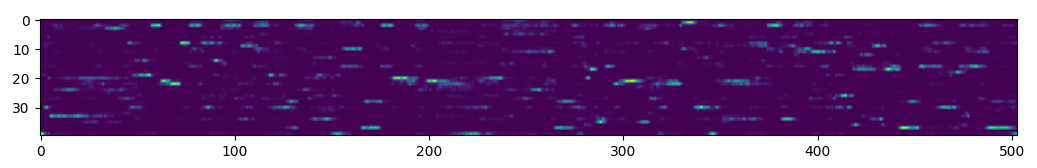
\includegraphics[width=\textwidth]{img/ppg_ant.png}
\item A Sanderson PPG representing the utterance \textit{``Geometric algebra, that is a whole other topic, uh, 
potentially for another day, but that's a - that's a really valid qustion''}:\\
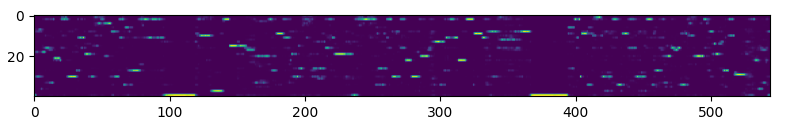
\includegraphics[width=\textwidth]{img/ppg_san.png}
\end{itemize}
    \subsection{Transcriptions [1]}
        The transcription process made use of a hybrid process. Analogously to the gain in speed reported in 
machine-assisted translation, it is faster to correct automatically-generated transcriptions than it is to 
manually create all transcriptions from scratch.

First, transcriptions were generated automatically by the Python library Allosaurus. 
These were only moderately accurate, and due to the nature of the Connectionist Temporal Classification 
loss which which the model is trained, the output sequence cannot have 
repeating tokens. Additionally, word boundaries were not included. This lack of word boundaries was 
hypothesized to be disadvantageous for speech synthesis, especially because the standard Tacotron 2 model 
input includes spaces and (standardized) punctuation.

Because of this, transcriptions were corrected by hand. Word boundaries were added, denoted by the underscore 
character (\texttt{\_}). Additionally, the removal of repeated phones in different words was corrected. 
For example, the phrase ``\textit{that takes some more rice}'' would be transcribed as 
\textipa{[D}
\textipa{\ae}
\textipa{t}
\textipa{e}
\textipa{k}
\textipa{s}
\textipa{2}
\textipa{m}
\textipa{o}
\textipa{\*r}
\textipa{a}
\textipa{I}
\textipa{s]}.
Following the manual correction, the transcription would be 
\textipa{[D}
\textipa{\ae}
\textipa{t}
\textipa{\_}
\textipa{t}
\textipa{e}
\textipa{k}
\textipa{s}
\textipa{\_}
\textipa{s}
\textipa{2}
\textipa{m}
\textipa{\_}
\textipa{m}
\textipa{o}
\textipa{\*r}
\textipa{\_}
\textipa{\*r}
\textipa{a}
\textipa{I}
\textipa{s]}.
Intuitively, it appears clear that the second transcription contains more information that 
would be relevant for IPA-to-speech synthesis.

Because successful automatic synthesis requires many examples of each input token, for each speaker 
the rarest IPA segments were removed and replaced with the best more common alternative, 
leaving only those segments occurring at least 20 times in the fine-tuning set of 200 utterances.

To improve the automatically-generated transcriptions, the pretrained models released by the authors 
of XX were fine-tuned on 200 manually corrected transcriptions each. Subsequently, an additional XX 
utterances were transcribed for each speaker, creating two datasets with XX utterances each.

%a
%æ
%ɑ
%b
%d
%ð
%d͡ʒ
%e
%ə
%ɛ
%f
%ɡ
%h
%i
%ɪ
%j
%k
%l
%m
%n
%ŋ
%o
%ɔ
%p
%ɹ
%ɹ̩
%s
%ʃ
%t
%t͡ʃ
%u
%ʊ
%v
%ʌ
%w
%z
%ʒ
%θ

\newpage
\begin{center}
  \textbf{Phonetic Inventories}\\~\\
  \begin{tabular}{llcc}
    Phone               & Definition                           & Antonimuthu & Sanderson \\\hline
    a                   & open front unrounded vowel           & \checkmark  & \checkmark \\
    \ae                 & near-open front unrounded vowel      & \checkmark  & \checkmark \\
    \textipa{A}         & open back unrounded vowel            & \checkmark  & \checkmark \\
    \textipa{6}         & open back rounded vowel              & \checkmark  &            \\
    b                   & voiced bilabial plosive              & \checkmark  & \checkmark \\
    d                   & voiced alveolar plosive              & \checkmark  & \checkmark \\
    \textipa{D}         & voiced dental fricative              & \checkmark  & \checkmark \\
    \textdyoghlig       & voiced post-alveolar affricate       & \checkmark  & \checkmark \\
    \textipa{\:d}       & voiced retroflex plosive             & \checkmark  &            \\
    e                   & close-mid front unrounded vowel      & \checkmark  & \checkmark \\
    \textipa{@}         & mid central vowel (schwa)            & \checkmark  & \checkmark \\
    \textipa{E}         & open-mid front unrounded vowel       & \checkmark  & \checkmark \\
    f                   & voiceless labiodental fricative      & \checkmark  & \checkmark \\
    g                   & voiced velar stop                    & \checkmark  & \checkmark \\
    h                   & voiceless glottal fricative          & \checkmark  & \checkmark \\
    i                   & close front unrounded vowel          & \checkmark  & \checkmark \\
    \textipa{I}         & near-close front unrounded vowel     & \checkmark  & \checkmark \\
    \textipa{1}         & close central unrounded vowel        & \checkmark  &            \\
    j                   & voiced palatal approximant (yod)     & \checkmark  & \checkmark \\
    \textipa{J}         & voiced palatal fricative             & \checkmark  &            \\
    \textbardotlessj    & voiced palatal plosive               & \checkmark  &            \\
    k                   & voiceless velar plosive              & \checkmark  & \checkmark \\
    \textipa{k\super h} & aspirated voiceless velar plosive    & \checkmark  &            \\
    l                   & voiced alveolar lateral approximant  & \checkmark  & \checkmark \\
    \textipa{\|[l}      & voiced dental approximant            & \checkmark  &            \\
    m                   & voiced bilabial nasal                & \checkmark  & \checkmark \\
    
    
  \end{tabular}
\end{center}
\newpage
\begin{center}
  \textbf{Phonetic Inventories (cont.)}\\~\\
  \begin{tabular}{llcc}
    Phone               & Definition & Antonimuthu                  & Sanderson \\\hline
    n                   & voiced alveolar nasal                     & \checkmark & \checkmark \\
    \textipa{\:n}       & voiced retroflex nasal                    & \checkmark & \\
    \textipa{N}         & voiced velar nasal                        & \checkmark & \\
    o                   & close-mid back rounded vowel              & \checkmark & \checkmark \\
    \textipa{O}         & open-mid back rounded vowel               & \checkmark & \checkmark \\
    p                   & voiceless bilabial plosive                & \checkmark & \checkmark \\
    r                   & voiced alveolar trill                     & \checkmark & \\
    \textipa{\*r}       & voiced alveolar approximant               &            & \checkmark \\
    \textipa{\s{\*r}}   & syllabic voiced alveolar approximant      & \checkmark & \\
    \textipa{R}         & voiced alveolar tap/flap                  & \checkmark & \\
    s                   & voiceless alveolar fricative              & \checkmark & \checkmark \\
    \textipa{\:s}       & voiceless retroflex fricative             & \checkmark & \\
    \textipa{S}         & voiceless postalveolar fricative          & \checkmark & \checkmark \\
    t                   & voiceless alveolar plosive                & \checkmark & \checkmark \\
    \textipa{t\super h} & aspirated voiceless alveolar plosive      & \checkmark & \\
    \textteshlig        & voiceless palato-alveolar affricate       & \checkmark & \checkmark \\
    \textipa{\:t}       & voiceless retroflex plosive               & \checkmark & \\
    u                   & close back rounded vowel                  & \checkmark & \checkmark \\
    \textipa{U}         & near-close back rounded vowel             & \checkmark & \checkmark \\
    v                   & voiced labiodental fricative              & \checkmark & \checkmark \\
    \textipa{2}         & open-mid back unrounded vowel             & \checkmark & \checkmark \\
    w                   & voiced labial-velar approximant           & \checkmark & \checkmark \\ 
    x                   & voiceless velar fricative                 & \checkmark & \\ 
    z                   & voiced alveolar fricative                 & \checkmark & \checkmark \\ 
    \textipa{\:z}       & voiced retroflex sibilant fricative       & \checkmark & \checkmark \\ 
    \textipa{Z}         & voiced postalveolar fricative             &            & \checkmark \\
    \textipa{T}         & voiceless dental (non-sibilant) fricative &            & \checkmark \\
  \end{tabular}
\end{center}
\section{Results [4]} % [4]
    \subsection{Continuous Representation-Based Speech Synthesis and Accent Transfer}
        The usefulness of pre-synthesis transformation of PPGs requires that there be a systematic difference between
the PPGs of speaker A and speaker B. Empirically, this was not the case, as the loss of each classifier 
converged around $0.69$ with only small and apparently random fluctuations even after hundreds of epochs. 
This value is approximately the expected loss of binary cross entropy on random data,
or $-\textrm{ln} \frac{1}{2} \approx 0.693147$. Thus, we can confidently conclude that there is no systematic 
difference between the PPGs of Sanderson and Antonimuthu.

While disappointing, this finding was not entirely uninteresting. It suggests that, at least at the 
resolution of 40 phonemes, even speakers speaking the same language with starkly contrasting accents 
will have their speech mapped into a common phonetic space, in which the respective phonetic representations 
are indistinguishable.

A further disappointing finding was that speech synthesis from 40-phone PPGs was not able to generate coherent 
speech for the Sanderson and Antonimuthu corpora. Because Waveglow generated comprehensible speech from mel spectrograms, 
this was clearly due to the generation of mel spectrograms from PPGs. This falsifies the original hypothesis that 
high-quality speech synthesis from 40-phone PPGs is possible. 

While the ``black box'' nature of neural networks makes it impossible at this point to draw conclusions about 
the causes of this failure with any certainty, there are two factors that seem most likely. First, it may be 
that the 40-phone PPGs simply do not carry sufficient information. As described above [XXX] succeeded in 
generating high-quality speech from 5860-dimensional PPGs. The reduction by more than two orders of magnitude may 
simply too large a reduction.

Secondly, the nature of the data in the respective speech corpora is, despite the data cleaning process, 
noisier and less uniform than standard corpora used in speech synthesis, such as LJSpeech. This is primarily 
due to the spontaneous nature of the speech, which is is more difficult to re-create with a neural network 
than speech read by a professional voice actor.
    \subsection{Transcription-Based Speech Synthesis and Accent Transfer}
        \input{sections/06_02_transcription_results.tex}
\section{Conclusions} % [3]
        %Possibility of IPA speech synthesis?
%Possibility of GANs on intermediate represenation?
%Possibility of speech synthesis involving spontaneous speech?
% --> need to annotate pauses
%

It should be noted that this work does not make any normative prescriptions about a ``correct'' dialect of English,
nor does it condone such prescriptions. In the author's view, different dialects are equally valid.
Applications of accent transfer, such as accent reduction, may be motivated by practical concerns, such as the desire to decrease the difficulty 
of understanding or being understood by an interlocutor. However, these considerations do not imply the superiority 
of any accent over another. The focus on one of the two theoretically possible directions of transfer, 
namely Indian English to American English, was motivated by considerations regarding the phones available in each.

This work, unfortunately, was not able to improve upon the results of XXX regarding speech synthesized from PPGs. However, an interesting direction 
for future work might be to work with multi-accent or even multi-language acoustic models. Conceivably, 
speakers with different accents would be distinguishable in such a phonetic space, rendering the transfer models 
more useful.

The two most interesting novel contributions in this work are the demonstration of speech synthesis from 
IPA, and the presentation of a method for transcription-to-transcription mappings.

*** TO BE ADDED - WAITING FOR RESULTS ***

\bibliographystyle{plainnat}
\bibliography{references}
\end{document}